\PassOptionsToPackage{svgnames}{xcolor}
\documentclass[
	8pt,
	xcolor=table,
	aspectratio=169,
	professionalfonts,
	ignorenonframetext,
	hyperref={
			pdfencoding=auto,
			linktocpage=true,
			colorlinks=true,
			linkcolor=DarkBlue,
			urlcolor=magenta,
			pdfpagelabels%	bookmark=false
		}
]{beamer}

\usepackage[breakable]{tcolorbox} % most
\useinnertheme{tcolorbox}
\tcbset{breakable,title after break=\insertblocktitle}

\usepackage[ngerman,english]{babel}

\usepackage{mathtools}
\usepackage[ISO]{diffcoeff}
\usepackage{dsfont}

\graphicspath{{images/}}

\let\oldforall\forall
\renewcommand{\forall}{\oldforall \, }
\let\oldexist\exists
\renewcommand{\exists}{\oldexist \: }
\newcommand\existu{\oldexist! \: }

\usepackage[
	% citestyle=numeric,
	% style=amsplain,
	% backend=biber,
	% defernumbers=true,
	% sorting=ynt,
	% maxcitenames=4
]{biblatex}
\addbibresource{references.bib}


\usepackage{bookmark}
% \usepackage[
% 	audience=english
% 	audience=spanish
% 	audience=german
% ]{beameraudience}

\setbeamersize{text margin left=5pt,text margin right=5pt}
% \setbeameroption{show notes on second screen}
\setbeamertemplate{note page}{\insertnote}
\usefonttheme[onlymath]{serif}

\setbeamertemplate{navigation symbols}{}
\setbeamertemplate{footline}[frame number]{}
\setbeamertemplate{headline}{}
\setbeamertemplate{items}[ball]
%\setbeamertemplate{blocks}[rounded][shadow=false]
\addtobeamertemplate{block begin}{\setlength\abovedisplayskip{0pt}}

\setbeamertemplate{bibliography item}{%
	\ifboolexpr{ test {\ifentrytype{book}} or test {\ifentrytype{mvbook}}
		or test {\ifentrytype{collection}} or test {\ifentrytype{mvcollection}}
		or test {\ifentrytype{reference}} or test {\ifentrytype{mvreference}} }
	{\setbeamertemplate{bibliography item}[book]}
	{\ifentrytype{online}
		{\setbeamertemplate{bibliography item}[online]}
		{\setbeamertemplate{bibliography item}[article]}}%
	\usebeamertemplate{bibliography item}}

\defbibenvironment{bibliography}
{\list{}
	{\settowidth{\labelwidth}{\usebeamertemplate{bibliography item}}%
		\setlength{\leftmargin}{\labelwidth}%
		\setlength{\labelsep}{\biblabelsep}%
		\addtolength{\leftmargin}{\labelsep}%
		\setlength{\itemsep}{\bibitemsep}%
		\setlength{\parsep}{\bibparsep}}}
{\endlist}
{\item}

\title{
	\huge\sffamily\color{DarkBlue}
	\href{https://github.com/carlosal1015/stone-weierstrass}{The Stone – Weierstraß Theorem}
	\vspace{2cm}
}

\author[C. Aznarán Laos]{
	\color{DarkBlue}
	Carlos A. Aznarán Laos
}

\institute[FC – UNI]{
	\large\color{DarkBlue}
	Science Department \and
	National University of Engineering
}

\date{
	\color{DarkBlue}
	\today
}

\titlegraphic{
	\begin{picture}(0,0)
		\put(-75,150){\makebox(0,0)[rt]{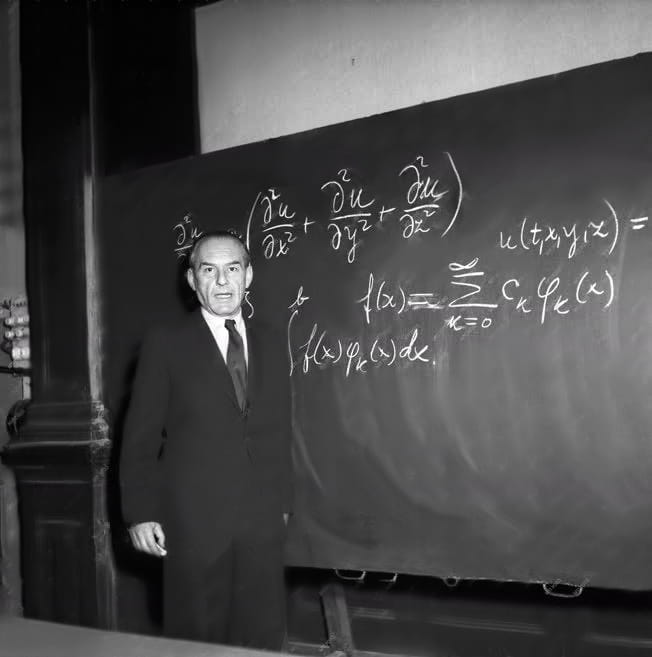
\includegraphics[width=5.2cm]{fejer}}}
		\put(220,170){\makebox(0,0)[rt]{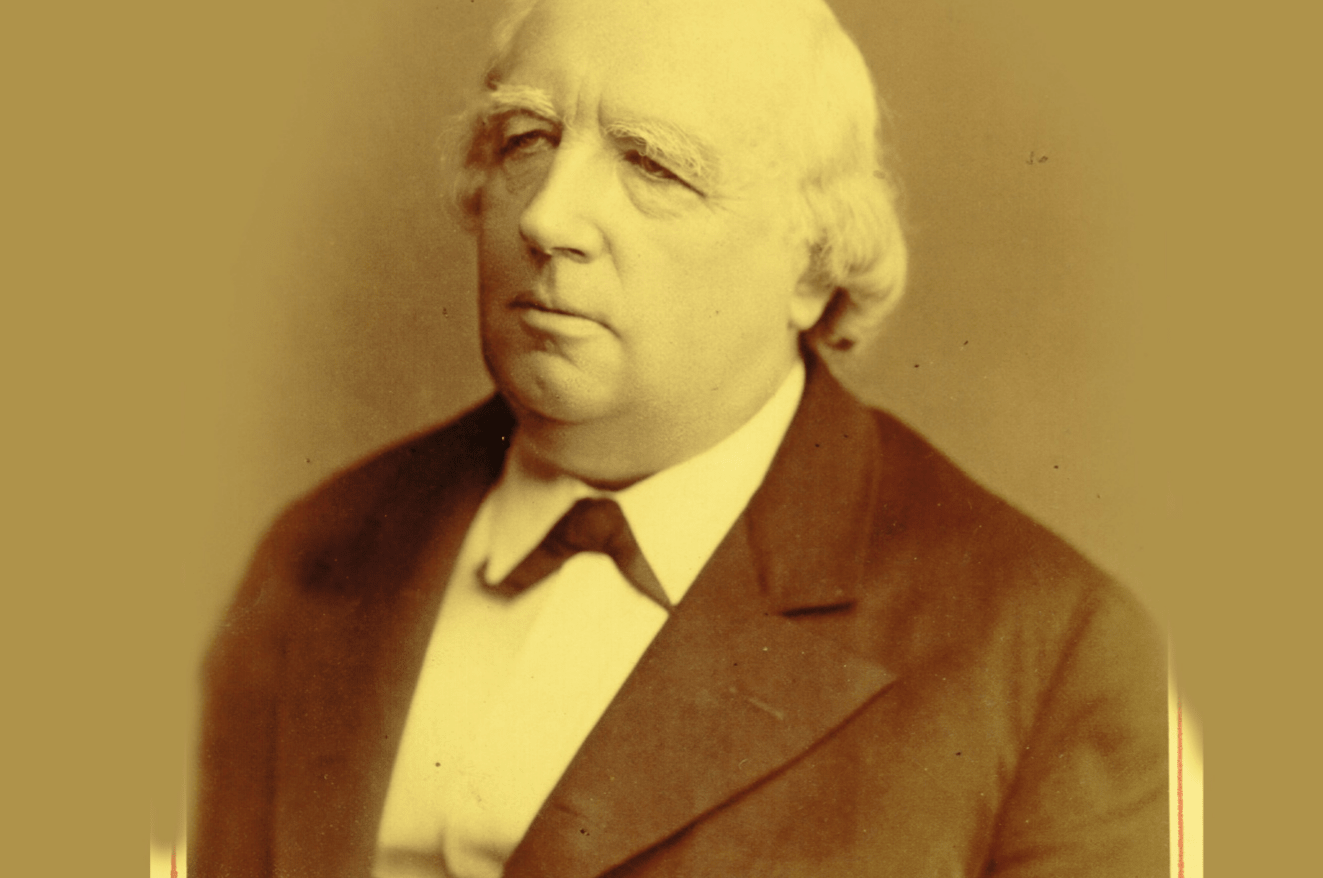
\includegraphics[width=5cm]{weierstrass}}}
		\put(220,80){\makebox(0,0)[rt]{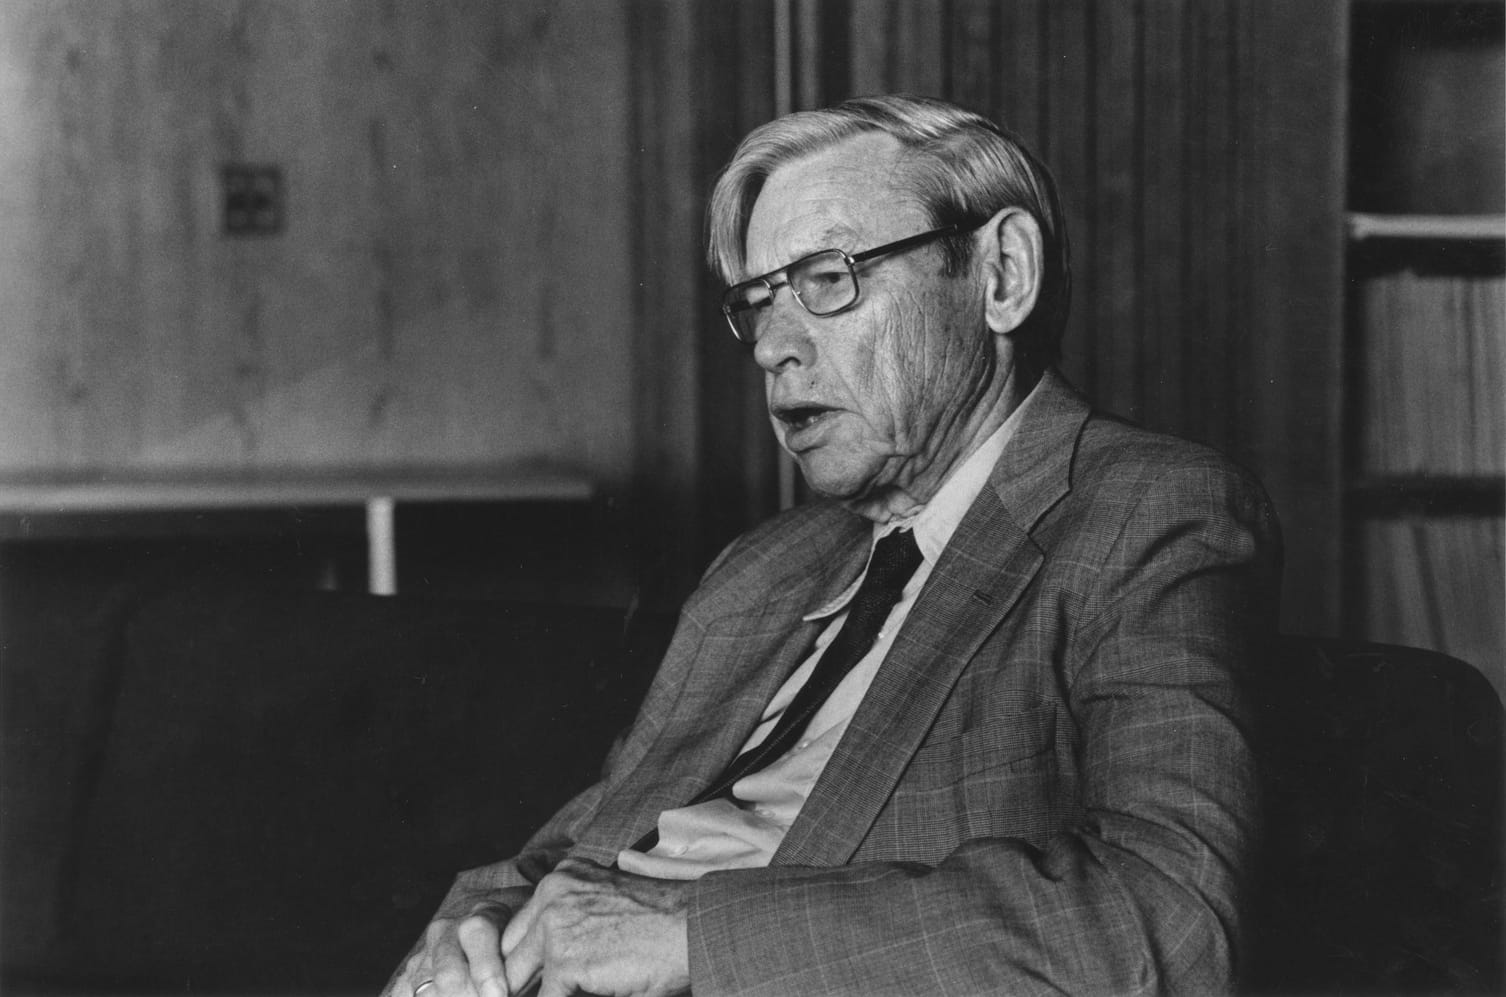
\includegraphics[width=5cm]{stone}}}
	\end{picture}
}